\documentclass[12pt]{article}

\title{Activity 3: Data Types}
\author{Chris Mayfield and Stoney Jackson}
\date{July 2017}

%\ProvidesPackage{cspogil}

% fonts
\usepackage[utf8]{inputenc}
\usepackage[T1]{fontenc}
\usepackage{mathpazo}

% spacing
\usepackage[margin=2cm]{geometry}
\renewcommand{\arraystretch}{1.4}
\setlength{\parindent}{0pt}

% orphans and widows
\clubpenalty=10000
\widowpenalty=10000
\pagestyle{empty}

% figures and tables
\usepackage{graphicx}
\usepackage{multicol}
\usepackage{tabularx}
\usepackage{wrapfig}

% fixed-width columns
\usepackage{array}
\newcolumntype{L}[1]{>{\raggedright\let\newline\\\arraybackslash\hspace{0pt}}m{#1}}
\newcolumntype{C}[1]{>{\centering\let\newline\\\arraybackslash\hspace{0pt}}m{#1}}
\newcolumntype{R}[1]{>{\raggedleft\let\newline\\\arraybackslash\hspace{0pt}}m{#1}}

% include paths
\makeatletter
\def\input@path{{Models/}{../../Models/}}
\graphicspath{{Models/}{../../Models/}}
\makeatother

% colors
\usepackage[svgnames,table]{xcolor}
\definecolor{bgcolor}{HTML}{FAFAFA}
\definecolor{comment}{HTML}{007C00}
\definecolor{keyword}{HTML}{0000FF}
\definecolor{strings}{HTML}{B20000}

% table headers
\newcommand{\tr}{\bf\cellcolor{Yellow!10}}

% syntax highlighting
\usepackage{textcomp}
\usepackage{listings}
\lstset{
    basicstyle=\ttfamily\color{black},
    backgroundcolor=\color{bgcolor},
    numberstyle=\scriptsize\color{comment},
    commentstyle=\color{comment},
    keywordstyle=\color{keyword},
    stringstyle=\color{strings},
    columns=fullflexible,
    keepspaces=true,
    showlines=true,
    showstringspaces=false,
    upquote=true
}

% code environments
\newcommand{\java}[1]{\lstinline[language=java]{#1}}%[
\lstnewenvironment{javalst}{\lstset{language=java,backgroundcolor=}}{}
\lstnewenvironment{javabox}{\lstset{language=java,frame=single,numbers=left}\quote}{\endquote}

% PDF properties
\usepackage[pdftex]{hyperref}
\urlstyle{same}
\makeatletter
\hypersetup{
  pdftitle={\@title},
  pdfauthor={\@author},
  pdfsubject={\@date},
  pdfkeywords={},
  bookmarksopen=false,
  colorlinks=true,
  citecolor=black,
  filecolor=black,
  linkcolor=black,
  urlcolor=blue
}
\makeatother

% titles
\makeatletter
\renewcommand{\maketitle}{\begin{center}\LARGE\@title\end{center}}
\makeatother

% boxes [optional height]
\newcommand{\emptybox}[1][10em]{
\vspace{1em}
\begin{tabularx}{\linewidth}{|X|}
\hline\\[#1]\hline
\end{tabularx}}

% models
\newcommand{\model}[1]{\section{#1}\nopagebreak}
\renewcommand{\thesection}{Model~\arabic{section}}

% questions
\newcommand{\quest}[1]{\subsection*{Questions~ (#1)}}
\newcounter{question}
\newcommand{\Q}{\vspace{1em}\refstepcounter{question}\arabic{question}.~ }
\renewcommand{\thequestion}{\#\arabic{question}}

% sub-question lists
\usepackage{enumitem}
\setenumerate[1]{label=\alph*)}
\setlist{itemsep=1em,after=\vspace{1ex}}

% inline answers
\definecolor{answers}{HTML}{C0C0C0}
\newcommand{\ans}[1]{%
\ifdefined\Student
    \leavevmode\phantom{~~\textcolor{answers}{#1}}
\else
    ~~\textcolor{answers}{#1}
\fi}

% longer answers [optional height]
\newsavebox{\ansbox}
\newenvironment{answer}[1][4em]{
\nopagebreak
\begin{lrbox}{\ansbox}
\begin{minipage}[t][#1]{\linewidth}
\color{answers}
}{
\end{minipage}
\end{lrbox}
\ifdefined\Student
    \phantom{\usebox{\ansbox}}%
\else
    \usebox{\ansbox}%
\fi}


\begin{document}

\maketitle

Java supports two main types of data: \emph{primitive types} like \java{int} and \java{double} that represent a single value, and \emph{reference types} like \java{String} and \java{Scanner} that represent more complex information.

\guide{
  \item Explain how POGIL roles improve team success.
  \item Name Java's primitive data types and give examples of each one.
  \item Identify illegal assignment statements, and explain why they are illegal.
  \item Describe what it means for variables to store a reference to an object.
}{
  \item Providing feedback on how well other team members are working. (Teamwork)
}{
This activity focuses on primitive types, literals, and assignment statements.
By the end of the activity, students will be able to identify the types of literals, identify illegal assignment statements, and trace a sequence of assignment statements and their effects in memory.

Question 5: If students are stumbling on the letters used in primitive literals (e.g., L and F), you might direct them back to Model 1 and have them read out loud the primitive types. Now is a good opportunity to introduce `float` as a (broken) floating-point data type and have students explain where the name `double` comes from.

Question 6 is good for report-out, allowing students to collectively develop a rule for when an assignment is allowed. It might be helpful to have a couple of assignment statements handy to challenge their definition if it is a little off. But be careful, examples like `short x = 3; byte y = 3; char c = 3;`, which are legal, may challenge their definition, but open a can of worms. If these issues come up, you'll need to explain that javac will check the range of the value, and if it is acceptable, allow the assignment; that means `byte z = 255;` will fail.

Model 2 introduces a standard technique for drawing diagrams of variables to show the difference between primitive and reference types. It may be helpful at this point to direct students to [Java Tutor](http://pythontutor.com/java.html) which draws similar diagrams (including stack frames). This tool also has options for "render all objects on the heap" (instead of inlining) and "use text labels for pointers" (instead of drawing arrows), which can help reinforce the concept of memory addresses. On \#14: have 2-3 teams draw their diagrams on the board and address common misconceptions.
}

\model{Primitive Types}
\label{CS1/primitive-types}

\vspace{-1ex}
\begin{table}[h!]
\begin{tabularx}{\linewidth}{|X|X|X|X|}
\hline
\tr Keyword    & \tr Size & \tr Min Value & \tr Max Value \\
\hline
\java{byte}    & 1 byte   & $-128$    & $127$ \\
\hline
\java{short}   & 2 bytes  & $-32,768$ & $32,767$ \\
\hline
\java{int}     & 4 bytes  & $-2^{31}$ & $2^{31}-1$ \\
\hline
\java{long}    & 8 bytes  & $-2^{63}$ & $2^{63}-1$ \\
\hline
\java{float}   & 4 bytes  & $\pm 3.4 \times 10^{-38}$  & $\pm 3.4 \times 10^{38}$ \\
\hline
\java{double}  & 8 bytes  & $\pm 1.7 \times 10^{-308}$ & $\pm 1.7 \times 10^{308}$ \\
\hline
\java{boolean} & N/A      & \java{false}     & \java{true} \\
\hline
\java{char}    & 2 bytes  & \java{'\\u0000'} & \java{'\\uffff'} \\
\hline
\end{tabularx}
\end{table}

Note that 1 byte is 8 bits, i.e., eight ``ones and zeros'' in computer memory.
Since there are only two options for each bit, with 8 bits you can represent $2^8 = 256$ possible values.


\quest{10 min}


\Q Which of the primitive types are integers? Which are floating-point? Which are not numeric?

\begin{answer}
\end{answer}


\Q Why do primitive types have ranges of values? What determines the range of the data type?

\begin{answer}
\end{answer}


\Q Why can't computers represent every possible number in mathematics? Will they ever be able to do so?

\begin{answer}
\end{answer}


\Q Since a \java{byte} can represent 256 different numbers, why is its max value 127 and not 128?

\begin{answer}
\end{answer}


\Q What is the data type for each of the following values?

\begin{quote}
\begin{multicols}{2}
1.14159 \ans{double} \\[1ex]
0       \ans{int} \\[1ex]
-1.0F   \ans{float} \\[1ex]
123     \ans{int}

7.2E-4  \ans{double} \\[1ex]
0.0     \ans{double} \\[1ex]
-13L    \ans{long} \\[1ex]
'0'     \ans{char}
\end{multicols}
\end{quote}


\Q Given the following variable declarations, which of the assignments are not allowed?

\begin{quote}
\begin{multicols}{2}

\begin{javalst}
byte miles;
short minutes;
int checking;
long days;
float total;
double sum;
boolean flag;
char letter;
\end{javalst}

\begin{javalst}
checking = 56000;
total = 0;
sum = total;
total = sum;
checking = miles;
sum = checking;
sum = days;
days = "0";
\end{javalst}

\end{multicols}
\end{quote}


\Q \label{allow} In general, when does Java allow you to assign one type of numeric variable to another?

\begin{answer}
\end{answer}


\Q Based on your answer to \ref{allow}, list all possible assignments in this format:
\java{int} $\gets$ \java{short}

\begin{answer}
\end{answer}

\newpage
\model{Reference Types}

\begin{quote}
\begin{minipage}{0.5\linewidth}

\begin{javalst}
int count;
double price;
String name;
Scanner in;

count = 0;
price = 1.99;
name = "Beyonce";
in = new Scanner(System.in);
\end{javalst}

\end{minipage}
\begin{minipage}{0.5\linewidth}

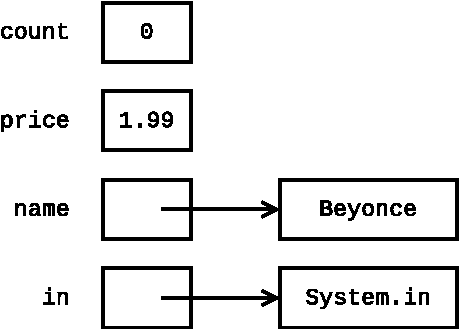
\includegraphics{CS1/reference1.pdf}

\end{minipage}
\end{quote}

Java has eight primitive types (see \ref{CS1/primitive-types}).
All other types of data are called \emph{reference} types, because \textbf{their value is a memory address}.
When drawing memory diagrams, use an arrow to \emph{reference} other memory locations (rather than make up integer values for the actual addresses).


\quest{10 min}


\Q What are the reference types in the example above?

\begin{answer}
\end{answer}


\Q In terms of style, what is the difference between primitive and reference type names?

\begin{answer}
\end{answer}


\Q Variables in Java can use at most eight bytes of memory. Explain why the values for Beyonce and System.in cannot be stored directly in the memory cells for \java{name} and \java{in}.

\begin{answer}
\end{answer}


\Q What is the value of the variable \java{count}? What is the value of the variable \java{price}?

\begin{answer}
\end{answer}


\Q What is the value of the variable \java{name}? What is the value of the variable \java{in}?

\begin{answer}
\end{answer}


\Q \label{assign} Carefully explain what it means to assign one variable to another. For example, what does the statement ~ \java{price = count;}~ do in terms of memory?

\begin{answer}
\end{answer}


\Q Draw a memory diagram for the following code. Make sure your answer is consistent with what you wrote for \ref{assign}.

\begin{javalst}
int width;
float score;
String first;
Scanner input;
String other;

width = 20;
score = 0.94;
first = "Taylor";
input = new Scanner(System.in);
score = width;
other = first;
\end{javalst}

\newpage
\model{Employability Skills}

``What do employers look for when they are seeking new college graduates to take on jobs?
According to NACE's \textit{Job Outlook 2016} survey, they are looking for leaders who can work as part of a team.''
{\footnotesize \url{http://www.naceweb.org/s11182015/employers-look-for-in-new-hires.aspx}}

\begin{table}[h!]
\centering

{\bf Attributes employers seek on a candidate's resume}
\vspace{2pt}

\renewcommand{\arraystretch}{1.0}
\begin{tabular}{|l|l|c|}
\hline
\tr & \tr Attribute   & \tr \% of respondents \\
\hline
1.  & Leadership                     & 80.1\% \\
\hline
2.  & Ability to work in a team      & 78.9\% \\
\hline
3.  & Communication skills (written) & 70.2\% \\
\hline
4.  & Problem-solving skills         & 70.2\% \\
\hline
5.  & Communication skills (verbal)  & 68.9\% \\
\hline
6.  & Strong work ethic              & 68.9\% \\
\hline
7.  & Initiative                     & 65.8\% \\
\hline
8.  & Analytical/quantitative skills & 62.7\% \\
\hline
9.  & Flexibility/adaptability       & 60.9\% \\
\hline
10. & Technical skills               & 59.6\% \\
\hline
\end{tabular}

%\vspace{1ex}
%\footnotesize
%Source: \textit{Job Outlook 2016}, National Association of Colleges and Employers
\end{table}
\vspace{-1em}


\quest{10 min}


\Q What is the relationship between the top two attributes employers seek?

\begin{answer}[3em]
Leadership implies working with other people, most likely as part of a team.
Working in teams is essential to developing leadership skills.
\end{answer}


\Q How is communication (written and verbal) related to problem-solving?

\begin{answer}[3em]
Solving problems in teams involves talking to other people and trying different approaches.
Writing solutions down is necessary to solidify the details and share them with others.
\end{answer}


\Q As a team, come up with a short description/example of each attribute.

\begin{quote}
\begin{multicols}{2}
1. \ans{leading a group of people} \\[1ex]
2. \ans{geting along well with others} \\[1ex]
3. \ans{writing and reading effectively} \\[1ex]
4. \ans{finding solutions creatively} \\[1ex]
5. \ans{speaking and listening effectively}

6. \ans{self-motivated to work hard} \\[1ex]
7. \ans{acting or taking charge early} \\[1ex]
8. \ans{analyzing data and reasoning} \\[1ex]
9. \ans{being able to handle change} \\[1ex]
10. \ans{computer/technology literacy}
\end{multicols}
\end{quote}


\Q Which of these skills do you expect to develop in this course? Why?

\begin{answer}[3em]
Ideally, all of them. Students will definitely learn technical computer programming skills.
But working in teams provides the opportunity to develop many other employable skills.
\end{answer}


\end{document}
